% !TeX root = ICCPS18.tex



%\scottC{the sub text in figure \ref{fig:microgrid} it is not clear. does the smart meter handle the billing or the DSO? Both?}


\section{Introduction}
%\Abhishek{I am going to use the publications of the Vermont guys - the quantised energy work to justify how we are setting up the framework}

%{\bf Emerging Trends:}
Power grids are undergoing major changes due to the
%an increase in the use of distributed energy resources (DER) and a 
rapid adoption of renewable energy resources, such as wind and solar power \cite{EIA2014,5430489}. For example, 
$4,\!143$ megawatts of solar panels were installed in the third quarter of 2016 \cite{seia}. This capacity is predicted to grow from 4\% of the total global energy production
%\AronC{4\% of what? I'm assuming total production in the US, but could be clarified.} 
in 2015 to 29\% in 2040 \cite{Randal}. Simultaneously, the battery technology costs per kWh have been dropping significantly \cite{stock2015powerful}, reaching grid parity \cite{bronski2015economics}. These trends are enabling a different vision for the future of power-grid operations: a decentralized system in which local communities are arranged in microgrids \cite{rahimi2012transactive}. In this vision, energy generation, transmission, distribution, and storage (i.e., electric vehicles or wall-mounted residential batteries) can be strategically used to balance load and demand spikes. A key feature of this vision is the support for local peer-to-peer energy trading within microgrids to reduce the load on the distribution system operators (DSO), leading to the development of Transactive Energy Systems (TES) \cite{kok2016society,cox2013structured,melton2013gridwise}. Such mechanisms 
can improve system reliability and efficiency by integrating inverter-based renewable resources into the grid and by supplying power to the local loads when the main grid is  interrupted. 


\begin{figure*}[t]
\centering
\vspace{-2.25em}
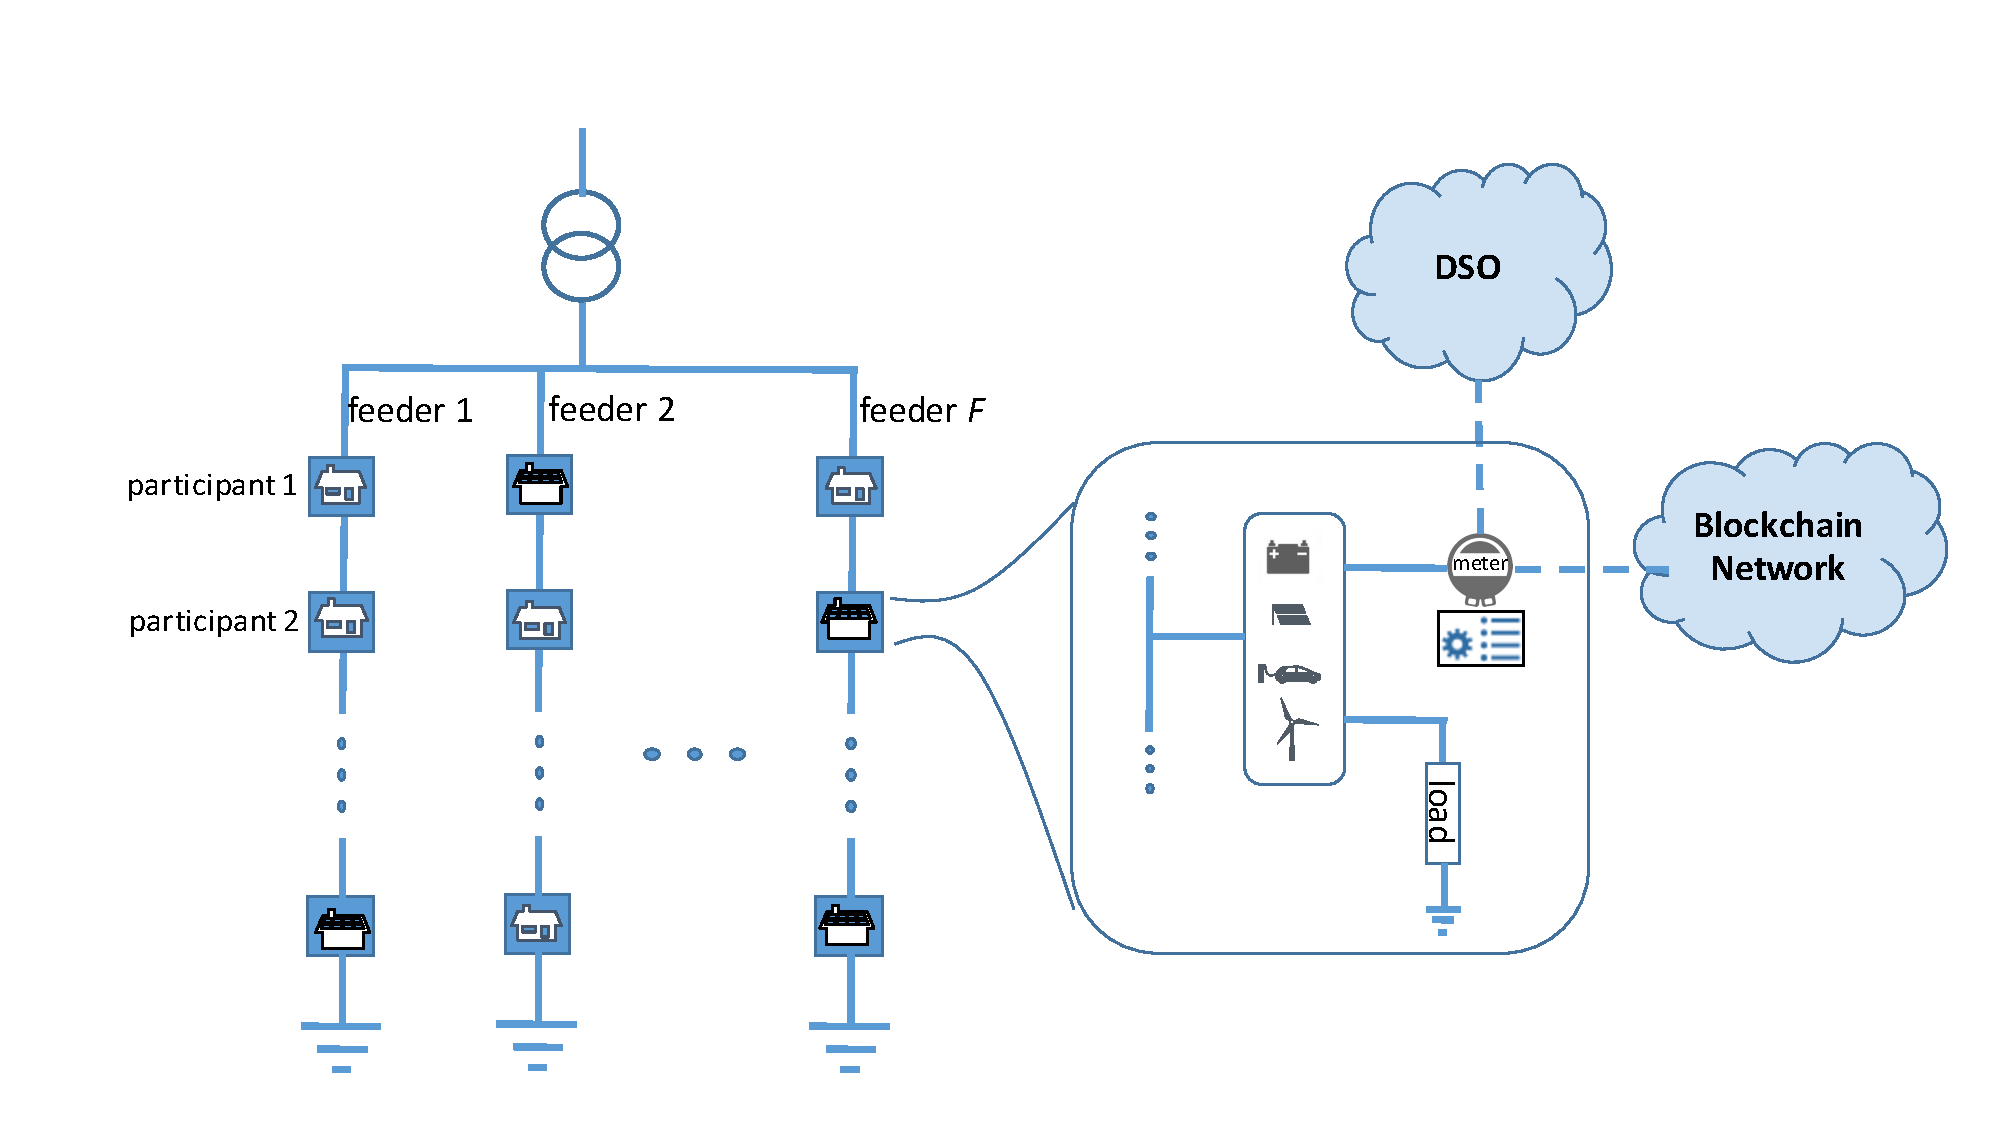
\includegraphics[width=0.75\textwidth]{diagrams/ProblemSetting}
\vspace{-1.25em}
\caption{We consider a multi-feeder microgrid. A feeder has number of nodes, some of whom have the capability to sell energy. Each feeder is protected by an overcurrent relay at the junction of the common bus. The inset figure shows that a node in the network has different kinds of loads, some of which can be scheduled, making it possible for a consumer to bid in advance for those loads. The smart meter ensures proper billing per node. The blockchain network is an immutable record of all transactions and is used for scheduling energy transfers between homes in the microgrid and between homes and the DSO.%and also by the Distribution System Operator (DSO) to produce a monthly bill.
}
\label{fig:microgrid}
\end{figure*}

This new vision of decentralized peer-to-peer energy market is synergistic with the recent advances and push towards Internet of Things, as shown by Volttron \cite{katipamula2016volttron},
OpenFMB \cite{gunthersmart}, and the Resilient Information
Architecture Platform for Smart Grid (RIAPS)
\cite{eisele2017riaps,Scott2017ICCPS}. The latter is a platform developed by our extended research team, and it provides foundations for all
algorithms, isolates the hardware details from the algorithms, and
provides essential mechanisms for resource management, fault
tolerance, and security.  

With the assumption of the availability of these new IoT platforms in the microgrid, we can develop appropriate transaction management platforms (TMPs) that allow  \emph{prosumers} (consumers who may also produce electricity) within a microgrid to participate freely in a local peer-to-peer energy trading market. With the advent and anticipated ubiquity of residential energy storage in the form of EVs or wall-mounted battery units \cite{Powerwall}, an important challenge is to design TMPs that allow for the efficient trade of \emph{energy futures}. However, the implementation of such TMPs remains difficult because of three integrated problems that must be addressed.



%These changes and the realization that the massive integration of renewable energy makes 



% This massive integration of renewable energy  makes it difficult
% to manage\AronC{Makes it difficult to manage what? Or what does it refer to?}, especially in the presence of variable distributed energy resources \cite{7452738}. Therefore, a different vision for the future of power-grid operations is emerging: a decentralized system in which local communities are arranged in microgrids \cite{rahimi2012transactive}. In this vision, energy generation, transmission, distribution, and storage (i.e., electric vehicles or wall-mounted residential batteries) can be strategically used to balance load and demand spikes. % Furthermore, distributed assets can provide the rest of the bulk power grid with ancillary services, including regulation and frequency response and supplemental reserves \cite{7725892}. 
%  Additionally, microgrids can improve system reliability and efficiency by integrating inverter-based renewable resources into the grid and by supplying power to the local loads when the main grid is  interrupted. 

%Furthering the concept of microgrids, transactive energy models have been proposed to support the next distribution system evolution \cite{kok2016society,cox2013structured,melton2013gridwise}.


%Transactive energy systems (TES) are defined as a set of market-based constructs for dynamically balancing the demand and supply across the electrical infrastructure \cite{melton2013gridwise}. \Karla{Considering the third point in next paragraph, we should emphasize trade of energy futures in this paragraph}.




%In this approach, customers on the same feeder \AronC{In our work, we also allow trading between feeders, so we might want to revise this sentence (e.g., ``customers in the same microgrid'').} (i.e. sharing a power line link) can operate in a P2P market, trading and exchanging generated energy locally. However, realization of this market is still difficult because of three integrated problems that must be addressed. 

The first problem relates to ensuring the physical stability and safety of the grid apparatus, and is mainly concerned with dynamically balancing supply and demand without violating line capacity constraints. The second is a distributed systems problem, which requires ensuring that this peer-to-peer market operates in a trustworthy manner even if some of the nodes are malicious. The third problem is related to privacy. 
While non-transactive smart metering systems require sharing prosumer information only with the DSO, transactive systems need to disseminate information among the participants to enable finding trade partners.
The dissemination of trading information threatens the privacy of prosumers since it  may expose their private information to anyone in the same microgrid. 
Further,
data collected from energy transactions is expected to be more fine-grained than data collected by currently deployed smart meters \cite{Privacy2017}, and may be used to infer personal information about the market participants. For example, a participant's presence or absence at their residence might be inferable from their energy future offers (e.g., if a prosumer posts an energy selling offer, the residents are less likely to be at home).
%\textcolor{red}{For example, a smart home may
%   know that its inhabitants will go out in the evening (\emph{e.g.},
%   by looking at their calendar), and it may trade energy futures
%   accordingly in the morning.  Without adequate privacy measures,
%   these trades may reveal to other prosumers in the microgrid that the
%   inhabitants will not be at home later.  
  Note that energy futures,
  whose delivery may happen several hours after  the transaction
  is made, can play an important role in predicting and controlling
  microgrid load.  In comparison, smart metering reveals only current
  (or past) usage.

%can be used to infer private information about the households

%On the one hand, design of transactive energy systems is a decentralized power system controls problem \cite{7452738}, requiring strategic microgrid control that maintains the stability of the community and the utility. On the other hand, it is a distributed market problem where erroneous as well as malicious transactions can create a gap between demand and supply, eventually destabilizing the system. 

%\Karla{Made changes to next three paragraphs. Small re-org}
In recent work \cite{Laszka17}, we have introduced {\it Privacy preserving Energy Transactions
(PETra)}, which is our distributed-ledger based solution that
(1) enables trading energy futures in a secure and verifiable
manner and (2) preserves prosumer privacy. 
Privacy in our previous work was implemented by using anonymized identifiers, a public distributed ledger, and a mixing service that prevents tracing the assets being traded back to the owner.
However, the transactive mechanism implemented in \cite{Laszka17} was opportunistic, where each consumer looked at the available asks from producers and chose the one that fit the needs of the consumer the best. In the present work, we consider an automated matching system that maximizes the amount of energy traded within the local market. Further, in the prior work, we did not consider system-wide safety constraints, only constraints on individual prosumers.

%\AronC{This paragraph seems a bit out of place.}
%In this paper, we consider a mechanism where energy is transferred at uniform power in discrete fixed-length intervals, which allows participants to plan their energy consumption and production. The company Packetized Energy \cite{packetizedenergy} has shown that selling power in discrete units is practical. However, their work requires  coordination from a centralized, trusted entity. As a result, they do not have to worry about the privacy challenges, which become apparent when we allow decentralized trades between entities.

%In the model considered in this paper, we assume that Distribution System Operators (DSOs) can act as custodians of this market, while still meeting the net demand in the microgrid \cite{7462854}. Thereafter, we consider the problem of decentralized trades, which use  the services of a distributed ledger to ensure that all events and transactions are tracked robustly through the entire system.
%However, due to a number of challenges, these services have been restricted in the present to some pilot programs like Demand/Response \cite{7462854}.  

Building on our work in \cite{Laszka17}, 
we continue to use a blockchain to implement parts of our proposed TMP design. The use of blockchains (i.e. distributed ledgers) for implementations of TMPs is in line with the recent trends in the research community and industry focused on transactive energy markets \cite{Lo3Patent,PowerLedger}.
%\AbhishekC{we need more references}\Karla{added powerledger}
Although disintermediation of trust is widely regarded as the primary feature of blockchain-based transaction systems \cite{SpectrumBC}, their use in TES is appealing also because they elegantly integrate the ability to immutably record the ownership and transfer of assets, with essential distributed computing services such as Byzantine fault-tolerant consensus on the ledger state as well as event chronology. The ability to establish consensus on state and timing is important in the context of TESs since these are envisioned to involve the participation of self-interested parties, interacting with one another via a distributed computing platform that executes the transaction management. %Moreover,  records kept on blockchain systems benefit from being fully auditable, immutable, and redundantly replicated at many nodes.




%\textcolor{red}{Advantages of blockchain: 1) does not require a trusted entity 2) fully auditable 3) decentralized. These properties are necessary because in a transactive microgrid: 1) we do not necessarily have a trusted entity locally at all times (microgrid might not be continuously connected to the Internet, and we do not necessarily have a trusted hardware platform locally) 2) everyone should be able to verify that no one (not even the distribution system operator (DSO)) has cheated in trading 3) fault tolerance (platform needs to be run by multiple nodes).}

%In the paper, we should first state these requirements/constraints, and then present blockchains as the obvious best solution.


%However, those solutions do not consider the impact of the electricity market on the controller responsible for the stability of the system. Neither do they consider the challenges of privacy for the prosumers participating in the market.

%\textcolor{red}{we must declare why a blockchain based technology is interesting.}
%\Aron{Advantages of blockchain: 1) does not require a trusted entity 2) fully auditable 3) decentralized. These properties are necessary because in a transactive microgrid: 1) we do not necessarily have a trusted entity locally at all times (microgrid might not be continuously connected to the Internet, and we do not necessarily have a trusted hardware platform locally) 2) everyone should be able to verify that no one (not even the DSO) has cheated in trading 3) fault tolerance (platform needs to be run by multiple nodes). In the paper, we should first state these requirements/constraints, and then present blockchains as the obvious best solution.}

%\Karla{Although disintermediation of trust is widely regarded as the main feature of blockchain-based transaction systems, their use in applications such transactive energy is desirable also because many represent an integrated, practical alternative to PBFT algorithms used to achieve consensus on data and event chronology for boundedly asynchronous distributed systems.}

%\Aron{Do blockchains have any advantage over PBFT other than supporting public platforms?}

%In recent work \cite{Laszka17}, we have introduced {\it Privacy preserving Energy Transactions
%(PETra)}, which is our distributed-ledger based solution that
%(1) enables trading energy futures in a secure and verifiable
%manner, (2) preserves prosumer privacy, and (3) enables distribution system operators to regulate trading and enforce the safety rules\AronC{I think that we should emphasize that PETra safety rules were imposed on individual prosumers, while in this paper, we can also impose rules on feeders.}.


\noindent{\bf Contribution}: Our contributions in this paper are as follows: %We make the following contributions in this~paper:
\begin{compactitem}
\item  We co-design an automated matching mechanism and a decentralized IoT-based transaction management platform, whose goal is to support the energy trading workflow while ensuring privacy of the prosumers (i.e., their identity) and the safety of the system (i.e. satisfaction of line capacity constraints). 
This design problem is challenging because there is a direct conflict between safety, privacy, and market efficiency.


%\item We design and implement an automated  matching mechanism that ensures safety , preserves prosumers' privacy\scottC{What specifically is kept private in this case?}, and promotes local trade and market efficiency. This design problem is challenging because there is a direct conflict between safety, privacy and market efficiency.\Karla{Recommend we de-emphasize design of matching mechanism (also I removed "auction" above) since our intent is not to compete against existing market designs. I recommend we emphasize that our matching mechanism/workflow is a "co-design" aimed at facilitating implementation, and specifically implementation that ensures privacy and safety. }
\item We allow prosumers to consider the effect of energy storage in batteries by enabling them to specify multiple time intervals in which they could trade energy, which is necessary for taking full advantage of batteries.
\item We describe the architecture and the protocol specification of our platform.
%and \AronC{We could remove this.}\textcolor{red}{discuss the challenges faced while building such a platform.}
Our solution combines the security and immutability of blockchain-based smart contracts with the efficiency of traditional computational platforms.
\item 
Finally, we present an experimental evaluation of the proposed TMP and the resulting market performance, with and without the availability of prosumer-owned battery storage. We consider total energy trade throughput as the market performance metric.
%Finally, we present an experimental evaluation of the proposed system and compare the effectiveness \scottC{what is market effectiveness? Power provided/power requested?} of the market with and without battery storage.\Karla{Consider: "Finally, we present an experimental evaluation of the proposed TMP and resulting market performance, with and without the availability of prosumer-owned battery storage. We consider total energy trade throughput as the market performance metric."}
\end{compactitem}
%describe the design and implement

% \textcolor{red}{In this paper, we  extend the work to implement an optimal  decentralized future trading mechanism that preserves privacy of the individual home owners, while following the safety constraints of the system\AronC{Another novel contribution compared to PETra (and some other related work) is allowing offers to specify multiple time intervals, which is necessary for taking full advantage of batteries.}.}

% \textcolor{red}{{\bf Contribution}: We design and implement an automated auction and matching mechanism that ensures safety (i.e. satisfaction of line capacity constraints), preserves privacy, and promotes local trade and market efficiency. This design problem is challenging because there is a direct conflict between safety and privacy on the one hand, \scottC{Isn't there a tradeoff between safety and privacy as well? This makes them sound like they're together.}\AronC{I agree, there is definitely a tradeoff between privacy and safety.} and market efficiency on the other. \st{A  second contribution of our work is a demonstration of the ability of the microgrid to be used as a regulation market by the DSO. That is, the microgrid follows an aggregated time variant demand signal throughout the day. Ability to closely regulate the demand curve enables efficient pre-planning of generation resources by the DSO. }}



%\Abhishek{
\noindent{\bf Outline:}  We present our transactive microgrid model and a review of requirements in Section \ref{sec:system}.
Then, we give an overview of the state of the art in Section \ref{sec:related}.
We formalize the energy trading problem in Section~\ref{sec:problem}.
%Two versions of the problem formulation are presented in sections \ref{sec:4a}, \ref{sec:4b} and \ref{sec:extendedProblem}. 
Our solution approach is described in Section \ref{sec:solution}. The implementation architecture is summarized in Section \ref{sec:tradingsystem}. We present results and discussions in Section \ref{sec:results}. Finally, we conclude the paper in Section \ref{sec:conclusion}.


% \begin{itemize}
% \item What is transactive microgrid. Why is it important and what are they key challenges. Describe existing transactive energy demonstrations.
% \item Describe the key architectural and algorithmic advances that have taken place already. And what are the missing gaps.
% \begin{itemize}
% \item Most works do not address trades of futures (i.e. Basar). If they do, the setting is simplistic in not considering offers that involve a logical ``or'' (i.e. allowing a participant to indicate the ability to provide or consume a certain level of power within \emph{any one} of a set of time slots), which limits market efficiency. 
% \end{itemize}
% \item Describe the problem being addressed, and motivate. (precise definition later)
% \begin{itemize}
% \item Design and implement an automated auction and matching mechanism that ensures safety (i.e. satisfaction of line capacity constraints), preserves privacy and promotes local trade and market efficiency. 
% \item This problem is interesting and challenging because there is a direct conflict between safety and privacy, and market efficiency. 
% \end{itemize}
% \item What have we done in the past and is this paper about. What are they results and lessons learned
% \begin{itemize}
% \item we introduced the problem formulation, 
% \item A second contribution of our work is demonstration of the ability of microgrid to be used as a regulation market by the DSO. That is, the microgrid follows an aggregated time variant demand signal throughout the day. Ability to closely regulate the demand curve enables efficient pre-planning of generation resources by the DSO.
% \end{itemize}
% \item What is the outline of the paper.
% \end{itemize}
 
% = All homes can be classified into feeder sets: F, Feedermembership function M:F\rightarrow 2^N maps the set of homes into feeders. Mp:F\rightarrow 2^P
% = For each feeder there exists an over current protection unit that sets the limit of total current flowing through the feeder. The limit is specified in terms of Integers (smart contract cannot do floats) L:F\rightarrow Z+.
% ==Each prosumer has the instantenous energy transfer, planned energy transfer written in terms of power. Controlling how much power is exchanged for how long controls the net energy transferred.
% === This limit puts a net constraint on total power being exchanged at any given time through the feeder. Thus 
% \sum_{DSO(f,t)+ \sum_{Mp(f,t)}} \leq l(f)
